%%% Preamble
\documentclass[paper=a4, fontsize=11pt]{scrartcl}

\usepackage[T1]{fontenc}
\usepackage{lmodern} %AGREGO1
\usepackage{fourier}
\usepackage[utf8]{inputenc}
%\usepackage[spanish]{babel}					% English language/hyphenation
<<<<<<< HEAD
=======

>>>>>>> origin/EJ_4



\usepackage{color}
\usepackage[protrusion=true,expansion=true]{microtype}	
\usepackage{amsmath}
\usepackage{amsfonts,amsthm} % Math packages
\usepackage[pdftex]{graphicx}	
\usepackage{url}
\usepackage{import}
\usepackage{multicol}

\usepackage[margin=2cm]{geometry}

% %%% Custom sectioning
\usepackage{sectsty}
\allsectionsfont{\normalfont \scshape}


%%% Custom headers/footers (fancyhdr package)
\usepackage{fancyhdr}
\pagestyle{fancyplain}

\fancyhead{}											% No page header
\fancyfoot[L]{}											% Empty 
\fancyfoot[C]{}											% Empty
\fancyfoot[R]{\thepage}									% Pagenumbering
\renewcommand{\headrulewidth}{0pt}			% Remove header underlines
\renewcommand{\footrulewidth}{0pt}				% Remove footer underlines
\setlength{\headheight}{13.6pt}


%%% Equation and float numbering
\numberwithin{equation}{section}		% Equationnumbering: section.eq#
\numberwithin{figure}{section}			% Figurenumbering: section.fig#
\numberwithin{table}{section}				% Tablenumbering: section.tab#


%%% Maketitle metadata
\newcommand{\horrule}[1]{\rule{\linewidth}{#1}} 	% Horizontal rule

%\usepackage{graphicx}
%\usepackage{color} 
%\usepackage[dvipsnames]{xcolor}
%\colorlet{purple}{purple}


    \usepackage{geometry} % Required to change the page size to A4
    \geometry{a4paper} % Set the page size to be A4 as opposed to the default US Letter

    \usepackage{mathtools, nccmath}
    
    \usepackage{tikz}
    \usetikzlibrary{matrix,calc}

    %isolated term
%#1 - Optional. Space between node and grouping line. Default=0
%#2 - node
%#3 - filling color
\newcommand{\implicantsol}[3][0]{
    \draw[rounded corners=3pt, fill=#3, opacity=0.3] ($(#2.north west)+(135:#1)$) rectangle ($(#2.south east)+(-45:#1)$);
    }


%internal group
%#1 - Optional. Space between node and grouping line. Default=0
%#2 - top left node
%#3 - bottom right node
%#4 - filling color
\newcommand{\implicant}[4][0]{
    \draw[rounded corners=3pt, fill=#4, opacity=0.3] ($(#2.north west)+(135:#1)$) rectangle ($(#3.south east)+(-45:#1)$);
    }

%group lateral borders
%#1 - Optional. Space between node and grouping line. Default=0
%#2 - top left node
%#3 - bottom right node
%#4 - filling color
\newcommand{\implicantcostats}[4][0]{
    \draw[rounded corners=3pt, fill=#4, opacity=0.3] ($(rf.east |- #2.north)+(90:#1)$)-| ($(#2.east)+(0:#1)$) |- ($(rf.east |- #3.south)+(-90:#1)$);
    \draw[rounded corners=3pt, fill=#4, opacity=0.3] ($(cf.west |- #2.north)+(90:#1)$) -| ($(#3.west)+(180:#1)$) |- ($(cf.west |- #3.south)+(-90:#1)$);
}

%group top-bottom borders
%#1 - Optional. Space between node and grouping line. Default=0
%#2 - top left node
%#3 - bottom right node
%#4 - filling color
\newcommand{\implicantdaltbaix}[4][0]{
    \draw[rounded corners=3pt, fill=#4, opacity=0.3] ($(cf.south -| #2.west)+(180:#1)$) |- ($(#2.south)+(-90:#1)$) -| ($(cf.south -| #3.east)+(0:#1)$);
    \draw[rounded corners=3pt, fill=#4, opacity=0.3] ($(rf.north -| #2.west)+(180:#1)$) |- ($(#3.north)+(90:#1)$) -| ($(rf.north -| #3.east)+(0:#1)$);
}

%group corners
%#1 - Optional. Space between node and grouping line. Default=0
%#2 - filling color
\newcommand{\implicantcantons}[2][0]{
    \draw[rounded corners=3pt, opacity=.3] ($(rf.east |- 0.south)+(-90:#1)$) -| ($(0.east |- cf.south)+(0:#1)$);
    \draw[rounded corners=3pt, opacity=.3] ($(rf.east |- 8.north)+(90:#1)$) -| ($(8.east |- rf.north)+(0:#1)$);
    \draw[rounded corners=3pt, opacity=.3] ($(cf.west |- 2.south)+(-90:#1)$) -| ($(2.west |- cf.south)+(180:#1)$);
    \draw[rounded corners=3pt, opacity=.3] ($(cf.west |- 10.north)+(90:#1)$) -| ($(10.west |- rf.north)+(180:#1)$);
    \fill[rounded corners=3pt, fill=#2, opacity=.3] ($(rf.east |- 0.south)+(-90:#1)$) -|  ($(0.east |- cf.south)+(0:#1)$) [sharp corners] ($(rf.east |- 0.south)+(-90:#1)$) |-  ($(0.east |- cf.south)+(0:#1)$) ;
    \fill[rounded corners=3pt, fill=#2, opacity=.3] ($(rf.east |- 8.north)+(90:#1)$) -| ($(8.east |- rf.north)+(0:#1)$) [sharp corners] ($(rf.east |- 8.north)+(90:#1)$) |- ($(8.east |- rf.north)+(0:#1)$) ;
    \fill[rounded corners=3pt, fill=#2, opacity=.3] ($(cf.west |- 2.south)+(-90:#1)$) -| ($(2.west |- cf.south)+(180:#1)$) [sharp corners]($(cf.west |- 2.south)+(-90:#1)$) |- ($(2.west |- cf.south)+(180:#1)$) ;
    \fill[rounded corners=3pt, fill=#2, opacity=.3] ($(cf.west |- 10.north)+(90:#1)$) -| ($(10.west |- rf.north)+(180:#1)$) [sharp corners] ($(cf.west |- 10.north)+(90:#1)$) |- ($(10.west |- rf.north)+(180:#1)$) ;
}

%Empty Karnaugh map 4x4
\newenvironment{Karnaugh}%
{
\begin{tikzpicture}[baseline=(current bounding box.north),scale=0.8]
\draw (0,0) grid (4,4);
\draw (0,4) -- node [pos=0.7,above right,anchor=south west] {BA} node [pos=0.75,below left,anchor=north east] {DC} ++(135:1);
%
\matrix (mapa) [matrix of nodes,
        column sep={0.8cm,between origins},
        row sep={0.8cm,between origins},
        every node/.style={minimum size=0.3mm},
        anchor=8.center,
        ampersand replacement=\&] at (0.5,0.5)
{
                       \& |(c00)| 00         \& |(c01)| 01         \& |(c11)| 11         \& |(c10)| 10         \& |(cf)| \phantom{00} \\
|(r00)| 00             \& |(0)|  \phantom{0} \& |(1)|  \phantom{0} \& |(3)|  \phantom{0} \& |(2)|  \phantom{0} \&                     \\
|(r01)| 01             \& |(4)|  \phantom{0} \& |(5)|  \phantom{0} \& |(7)|  \phantom{0} \& |(6)|  \phantom{0} \&                     \\
|(r11)| 11             \& |(12)| \phantom{0} \& |(13)| \phantom{0} \& |(15)| \phantom{0} \& |(14)| \phantom{0} \&                     \\
|(r10)| 10             \& |(8)|  \phantom{0} \& |(9)|  \phantom{0} \& |(11)| \phantom{0} \& |(10)| \phantom{0} \&                     \\
|(rf) | \phantom{00}   \&                    \&                    \&                    \&                    \&                     \\
};
}%
{
\end{tikzpicture}
}

%Empty Karnaugh map 2x4
\newenvironment{Karnaughvuit}%
{
\begin{tikzpicture}[baseline=(current bounding box.north),scale=0.8]
\draw (0,0) grid (4,2);
\draw (0,2) -- node [pos=0.7,above right,anchor=south west] {bc} node [pos=0.7,below left,anchor=north east] {a} ++(135:1);
%
\matrix (mapa) [matrix of nodes,
        column sep={0.8cm,between origins},
        row sep={0.8cm,between origins},
        every node/.style={minimum size=0.3mm},
        anchor=4.center,
        ampersand replacement=\&] at (0.5,0.5)
{
                      \& |(c00)| 00         \& |(c01)| 01         \& |(c11)| 11         \& |(c10)| 10         \& |(cf)| \phantom{00} \\
|(r00)| 0             \& |(0)|  \phantom{0} \& |(1)|  \phantom{0} \& |(3)|  \phantom{0} \& |(2)|  \phantom{0} \&                     \\
|(r01)| 1             \& |(4)|  \phantom{0} \& |(5)|  \phantom{0} \& |(7)|  \phantom{0} \& |(6)|  \phantom{0} \&                     \\
|(rf) | \phantom{00}  \&                    \&                    \&                    \&                    \&                     \\
};
}%
{
\end{tikzpicture}
}

%Empty Karnaugh map 2x2
\newenvironment{Karnaughquatre}%
{
\begin{tikzpicture}[baseline=(current bounding box.north),scale=0.8]
\draw (0,0) grid (2,2);
\draw (0,2) -- node [pos=0.7,above right,anchor=south west] {b} node [pos=0.7,below left,anchor=north east] {a} ++(135:1);
%
\matrix (mapa) [matrix of nodes,
        column sep={0.8cm,between origins},
        row sep={0.8cm,between origins},
        every node/.style={minimum size=0.3mm},
        anchor=2.center,
        ampersand replacement=\&] at (0.5,0.5)
{
          \& |(c00)| 0          \& |(c01)| 1  \\
|(r00)| 0 \& |(0)|  \phantom{0} \& |(1)|  \phantom{0} \\
|(r01)| 1 \& |(2)|  \phantom{0} \& |(3)|  \phantom{0} \\
};
}%
{
\end{tikzpicture}
}

%Defines 8 or 16 values (0,1,X)
\newcommand{\contingut}[1]{%
\foreach \x [count=\xi from 0]  in {#1}
     \path (\xi) node {\x};
}

%Places 1 in listed positions
\newcommand{\minterms}[1]{%
    \foreach \x in {#1}
        \path (\x) node {1};
}

%Places 0 in listed positions
\newcommand{\maxterms}[1]{%
    \foreach \x in {#1}
        \path (\x) node {0};
}

%Places X in listed positions
\newcommand{\indeterminats}[1]{%
    \foreach \x in {#1}
        \path (\x) node {X};
}

    \linespread{1.2} % Line spacing
    
    \setlength\parindent{0pt} % Uncomment to remove all indentation from paragraphs


\makeatletter

\providecommand{\tabularnewline}{\\}

%\usepackage{babel}


\makeatother

%\usepackage{babel}

\usepackage{tikz}
\usepackage{circuitikz} 	%Esto es lo que se necesita para los circuitos.
%\usepackage{siunitx}
%\usemodule[circuitikz]
%\usepackage{circuitikzgit}

\usepackage{multicol}

\usepackage{float}

%\makeatletter

\providecommand{\tabularnewline}{\\}

%THE FOLLOWING ARE CONFIGURATIONS FOR TODONOTES
\usepackage{todonotes,varwidth}
\makeatletter
\tikzstyle{diaanotestyle} = [
    draw=\@todonotes@currentbordercolor,
    fill=\@todonotes@currentbackgroundcolor,
    line width=0.5pt,
    inner sep = 0.8 ex,
    rounded corners=4pt,align=left,
   ]

\renewcommand{\@todonotes@drawInlineNote}{%
        {\begin{tikzpicture}[remember picture,baseline={(0,0)}]%
            \draw node[diaanotestyle,font=\@todonotes@sizecommand,anchor=base west]{%
               \begin{varwidth}[t]{10cm}
                \if@todonotes@authorgiven%
                    {\@todonotes@sizecommand \@todonotes@author:\,\@todonotes@text}%
                \else%
                    {\@todonotes@sizecommand \@todonotes@text}%
                \fi
                \end{varwidth}};%
            \end{tikzpicture}}%
       }%
\makeatother
%HERE ENDS THE CONFIGURATIONS FOR TODONOTES

%THE FOLLOWING ARE CONFIGURATIONS FOR LISTINGS (to insert code)
\usepackage{listings}

\definecolor{dkgreen}{rgb}{0,0.6,0}
\definecolor{gray}{rgb}{0.5,0.5,0.5}
\definecolor{mauve}{rgb}{0.58,0,0.82}

\lstset{frame=tb,
  language=Verilog,
  aboveskip=3mm,
  belowskip=3mm,
  showstringspaces=false,
  columns=flexible,
  basicstyle={\small\ttfamily},
  numbers=none,
  numberstyle=\tiny\color{gray},
  keywordstyle=\color{blue},
  commentstyle=\color{dkgreen},
  stringstyle=\color{mauve},
  breaklines=true,
  breakatwhitespace=true,
  tabsize=3
}
%HERE ENDS THE CONFIGURATIONS FOR LISTINGS

%NEEDED FOR THE lt2ti TOOL
\usepackage[compatibility,siunitx,  americanvoltages, americancurrents, europeanresistors, europeaninductors, americanports,%
  straightlabels, fetbodydiode, straightvoltages]{circuitikz}
\usepackage{tikz,amsmath, amssymb,bm,color,pgfkeys,siunitx,ifthen,ulem}
\usepackage{pgfplots}
\pgfplotsset{compat=1.14}
%END OF NEEDED FOR lt2ti TOOL

%THIS IS SO THAT REFERENCES CAN BE CLICKED
\usepackage{hyperref}
\hypersetup{
    colorlinks=true,
    linkcolor=blue,
    filecolor=magenta,      
    urlcolor=blue,
    citecolor=blue,    
}
%END OF REFERENCES

\begin{document}

\title{
	%\vspace{-1in}
	\usefont{OT1}{bch}{b}{n}
	\normalfont \normalsize \textsc{Instituto Tecnológico de Buenos Aires} \\ [25pt]
	\horrule{2pt} \\[0.4cm]
	\huge Trabajo Pr\'actico Nº 1 \\
	\horrule{2pt} \\[0cm]
\author{Grupo 1:\\\\Farall, Facundo\\Gaytan, Joaqu\'in\\Kammann, Lucas\\Maselli, Carlos\\ \\ }
\text{Electr\'onica III - 2019}
}
\date{\today} %ver si dejar la de today o poner fecha fija que sea August 2018
\pagenumbering{arabic}

\maketitle
\newpage



% The \input command appends the content of the file directly into the document.
<<<<<<< HEAD
%\section{Ejercicio 1}
Se realizó un programa bajo el nombre run.py, dentro de la carpeta EJ\_1 del proyecto, el cual calcula el rango y resolución para una cierta convención de números en punto fijo.
Recibe tres parámetros por línea de comando: un 1 o un 0 indicando si el sistema es signado, cantidad de bits de la parte entera, y cantidad de bits de la parte fraccionaria, en ese órden.
Ante algún error en el formato en que se le pasan los parámetros, o ya sea porque los mismos exceden las capacidades del programa, se imprimirá en pantalla el mensaje ERROR.
Los errores pueden estar ocasionados por alguna de las siguientes razones:
\begin{itemize}
    \item No se pasa ningún argumento.
    \item Los argumentos no son números enteros.
    \item Se pasa una cantidad de argumentos distinta a 3.
    \item El primer argumento (que indica si el sistema es signado o no) es distinto de 0 o 1.
\end{itemize}


\subsection{Limitaciones del programa}
También puede devolverse ERROR a causa de que la cantidad de bits asignados a la parte entera o a la fraccionaria exceden los límites del lenguaje utilizado para el programa.
El código se escribió en Python y se buscaron los casos límite para los cuales el programa deja de devolver valores con sentido:
\begin{itemize}
    \item La cantidad de bits de la parte entera debe ser menor o igual a 1023.
    \item La cantidad de bits de la parte fraccionaria debe se menor o igual a 1074.
\end{itemize}


\section{Ejercicio 2}

% El desarrollo de la primera expresión de 5 variables
% usando mintérminos se realiza en esta subsección
\subsection{Expresi\'on en mint\'erminos}

\subsubsection{Simplificación con Álgebra booleana}

\subsubsection{Simplificación con mapas de Karnaugh}

\subsubsection{Expresión desarrollada usando NOR}

\subsubsection{Circuitos lógicos}

% El desarrollo de la segunda expresión de 4 variables
% usando maxtérminos se realiza en esta subsección
\subsection{Expresi\'on en maxt\'erminos}

\subsubsection{Simplificación con Álgebra booleana}

\subsubsection{Simplificación con mapas de Karnaugh}

\subsubsection{Expresión desarrollada usando NOR}

\subsubsection{Circuitos lógicos}

=======
\section{Ejercicio 1}
Se realizó un programa bajo el nombre run.py, dentro de la carpeta EJ\_1 del proyecto, el cual calcula el rango y resolución para una cierta convención de números en punto fijo.
Recibe tres parámetros por línea de comando: un 1 o un 0 indicando si el sistema es signado, cantidad de bits de la parte entera, y cantidad de bits de la parte fraccionaria, en ese órden.
Ante algún error en el formato en que se le pasan los parámetros, o ya sea porque los mismos exceden las capacidades del programa, se imprimirá en pantalla el mensaje ERROR.
Los errores pueden estar ocasionados por alguna de las siguientes razones:
\begin{itemize}
    \item No se pasa ningún argumento.
    \item Los argumentos no son números enteros.
    \item Se pasa una cantidad de argumentos distinta a 3.
    \item El primer argumento (que indica si el sistema es signado o no) es distinto de 0 o 1.
\end{itemize}


\subsection{Limitaciones del programa}
También puede devolverse ERROR a causa de que la cantidad de bits asignados a la parte entera o a la fraccionaria exceden los límites del lenguaje utilizado para el programa.
El código se escribió en Python y se buscaron los casos límite para los cuales el programa deja de devolver valores con sentido:
\begin{itemize}
    \item La cantidad de bits de la parte entera debe ser menor o igual a 1023.
    \item La cantidad de bits de la parte fraccionaria debe se menor o igual a 1074.
\end{itemize}


%\section{Ejercicio 2}

% El desarrollo de la primera expresión de 5 variables
% usando mintérminos se realiza en esta subsección
\subsection{Expresi\'on en mint\'erminos}

\subsubsection{Simplificación con Álgebra booleana}

\subsubsection{Simplificación con mapas de Karnaugh}

\subsubsection{Expresión desarrollada usando NOR}

\subsubsection{Circuitos lógicos}

% El desarrollo de la segunda expresión de 4 variables
% usando maxtérminos se realiza en esta subsección
\subsection{Expresi\'on en maxt\'erminos}

\subsubsection{Simplificación con Álgebra booleana}

\subsubsection{Simplificación con mapas de Karnaugh}

\subsubsection{Expresión desarrollada usando NOR}

\subsubsection{Circuitos lógicos}

>>>>>>> 51cf850cb34e2f69c7df82c6b75434383373e1c3
\section{Ejercicio 3}
De los dos módulos pedidos para implementar en Verilog se tomó la decisión de realizar uno mediante las compuertas lógicas que lo componen, y otro a través de la descripción de su comportamiento (behavioural).
La razón detrás de esta decisión fue para hacer uso de las variantes provistas por Verilog, e interiorizarnos en su estilo de programación.

\subsection{Decoder de 4 salidas}
Esta implementación de un decoder de 4 salidas recibe una arreglo de 2 bits, que determinan cual de las cuatro salidas accionar.
La misma se realizó a través de lógica de compuertas, donde únicamente la combinación correcta de los dos bits de entrada, ponen a la salida con ese número, en 1 lógico.
Las relaciones lógicas son sencillas de comprender y quedan explicitadas en el mismo código.
A continuación se presenta el código en Verilog:
\begin{lstlisting}
    module decoder4out(coded, y0, y1, y2, y3);
        input [1:0] coded;
        output y0, y1, y2, y3;

        assign y0 = ~coded[1] & ~coded[0];
        assign y1 = ~coded[1] & coded[0];
        assign y2 = coded[1] & ~coded[0];
        assign y3 = coded[1] & coded[0];

    endmodule
\end{lstlisting}

\subsection{MUX de 4 entradas}
Esta implementación de un mux de 4 entradas recibe un arreglo de 4 bits con las 4 "fuentes", otro arreglo de 2 bits que hace las veces de selector, y cuenta con una salida de 1 bit.
La salida copiará el valor de la entrada determinada por el selector.
El módulo se logró mediante una descripción del comportamiento del mismo, en el cual se le especificó qué debía realizar ante cambios en alguna de sus entradas.
A continuación se presenta el código en Verilog:
\begin{lstlisting}
    module mux4in (x, sel, y);
        input [3:0] x;
        input [1:0] sel;                      // sel selects the exit (x[3], x[2], x[1], x[0]).
        output reg y;

        always @(sel or x) begin
            if (sel == 0)
                assign y = x[0];
            else if (sel == 1)
                assign y = x[1];
            else if (sel == 2)
                assign y = x[2];
            else if (sel == 3)
                assign y = x[3];

        end

    endmodule
\end{lstlisting}

\subsection{Test-bench}
Se sometió a los dos módulos a un testeo de su respuesta a cada una de las posibles entradas, y los resultados fueron los esperados.
Los mismos pueden ser replicados ejecutando los comandos:
\begin{lstlisting}[language=bash]
    user@computer: path/to/EJ_3/folder$ make
    user@computer: path/to/EJ_3/folder$ ./run
\end{lstlisting}
\section{Ejercicio 4}

\subsection{Tabla de verdad}
En la siguiente tabla se muestra la equivalencia entre un n\'umero binario de 4 bits y el mismo en c\'odigo de Gray. Seg\'un la convenci\'on adpotada, "A" ser\'a el MSB y "D" ser\'a el LSB.

\begin{table}[H]\caption{Tabla de verdad}
\centering
\begin{tabular}{cccc|cccc}
A & B & C & D & $s_{1}$ & $s_{2}$ & $s_{3}$ & $s_{4}$ \\ \hline
0 & 0 & 0 & 0 & 0  & 0  & 0  & 0  \\
0 & 0 & 0 & 1 & 0  & 0  & 0  & 1  \\
0 & 0 & 1 & 0 & 0  & 0  & 1  & 1  \\
0 & 0 & 1 & 1 & 0  & 0  & 1  & 0  \\
0 & 1 & 0 & 0 & 0  & 1  & 1  & 0  \\
0 & 1 & 0 & 1 & 0  & 1  & 1  & 1  \\
0 & 1 & 1 & 0 & 0  & 1  & 0  & 1  \\
0 & 1 & 1 & 1 & 0  & 1  & 0  & 0  \\
1 & 0 & 0 & 0 & 1  & 1  & 0  & 0  \\
1 & 0 & 0 & 1 & 1  & 1  & 0  & 1  \\
1 & 0 & 1 & 0 & 1  & 1  & 1  & 1  \\
1 & 0 & 1 & 1 & 1  & 1  & 1  & 0  \\
1 & 1 & 0 & 0 & 1  & 0  & 1  & 0  \\
1 & 1 & 0 & 1 & 1  & 0  & 1  & 1  \\
1 & 1 & 1 & 0 & 1  & 0  & 0  & 1  \\
1 & 1 & 1 & 1 & 1  & 0  & 0  & 0
\end{tabular}
\end{table}

En base a esto, se puede expresar a cada bit de salida ($s_{1}$,$s_{2}$,$s_{3}$,$s_{4}$) como una combinaci\'on de entradas (A,B,C,D) en forma de minit\'erminos.

De esta forma, obtenemos las siguientes expresiones:

\begin{equation}\label{s1_mini}
    s_{1} = A.\overline{B}.\overline{C}.\overline{D} +A.\overline{B}.\overline{C}.D+A.\overline{B}.C.\overline{D}+A.\overline{B}.C.D+A.B.\overline{C}.\overline{D}+A.B.\overline{C}.D+A.B.C.D
\end{equation}

\begin{equation}\label{s2_mini}
    s_{2} = A\overline{B}\overline{C}\overline{D} +A\overline{B}\overline{C}D+A\overline{B}C\overline{D}+A\overline{B}CD+AB\overline{C}\overline{D}+AB\overline{C}D+ABCD
\end{equation}

\begin{equation}\label{s3_mini}
    s_{3} = \overline{A}\overline{B}C\overline{D}+\overline{A}\overline{B}CD+\overline{A}B\overline{C}\overline{D}+\overline{A}B\overline{C}D+A\overline{B}C\overline{D}+A\overline{B}CD+AB\overline{C}\overline{D}+AB\overline{C}D
\end{equation}

\begin{equation}\label{s4_mini}
    s_{4} = \overline{A}\overline{B}\overline{C}D+\overline{A}\overline{B}C\overline{D}+\overline{A}B\overline{C}D+\overline{A}BC\overline{D}++A\overline{B}\overline{C}D+A\overline{B}C\overline{D}+AB\overline{C}D+ABC\overline{D}
\end{equation}

\subsection{Simplificaci\'on. Mapas de Karnaugh}

Las expresiones calculadas en el apartado anterior no son del todo eficientes a la hora de implementar el circuito l\'ogico, debido a que no est\'an apropiadamente simplificadas. Para encontrar la expresi\'on \'optima que satisfaga la tabla de verdad utilizaremos el m\'etodo de mapas de Karnaugh, en este caso con minit\'erminos. Como tenemos cuatro salidas distintas debemos realizar cuatro de estos mapas, que resultar\'an en una expresi\'on de suma de productos de las entradas. A continuaci\'on se reproducen estos diagramas y las expresiones derivadas de los mismos, donde en cada mapa cada color representa un grupo.

\begin{center}

    \begin{Karnaugh}\label{Karnaugh_s1}
        \contingut{0,0,1,1,0,0,1,1,0,0,1,1,0,0,1,1}
       \implicant{3}{10}{red}
    \end{Karnaugh}

Mapa de Karnaugh para $s_1$

\begin{Karnaugh}\label{Karnaugh_s2}
        \contingut{0,1,1,0,0,1,1,0,0,1,1,0,0,1,1,0}
       \implicant{1}{9}{green}
       \implicant{2}{10}{red}
    \end{Karnaugh}

Mapa de Karnaugh para $s_2$

\begin{Karnaugh}\label{Karnaugh_s3}
        \contingut{0,1,0,1,0,1,0,1,1,0,1,0,1,0,1,0}
       \implicant{1}{7}{red}
       \implicantcostats{12}{10}{green}
     \end{Karnaugh}

Mapa de Karnaugh para $s_3$

\begin{Karnaugh}\label{Karnaugh_s4}
        \contingut{0,0,0,0,1,1,1,1,1,1,1,1,0,0,0,0}
       \implicant{4}{6}{red}
       \implicant{8}{10}{green}
    \end{Karnaugh}

Mapa de Karnaugh para $s_4$
\end{center}
Realizando las correspondientes asociaciones obtenemos las siguientes expresiones que describen el comportamiento de cada bit de salida.

\begin{equation}\label{s1_Karnaugh}
    s_{1}= A
\end{equation}

\begin{equation}\label{s2_Karnaugh}
    s_{2}= A.\overline{B}+\overline{A}.B
\end{equation}

\begin{equation}\label{s3_Karnaugh}
    s_{3}= B.\overline{C}+\overline{B}.C
\end{equation}

\begin{equation}\label{s4_Karnaugh}
    s_{4}= C.\overline{D}+\overline{C}.D
\end{equation}

\subsection{Circuito l\'ogico}\label{ej2_circ}

En base a las ecuaciones encontradas se construy\'o el circuito l\'ogico mostrado abajo, utilizando compuertas \textsc{OR}, \textsc{AND} y \textsc{NOT}.

\begin{figure}[H]
    \centering
    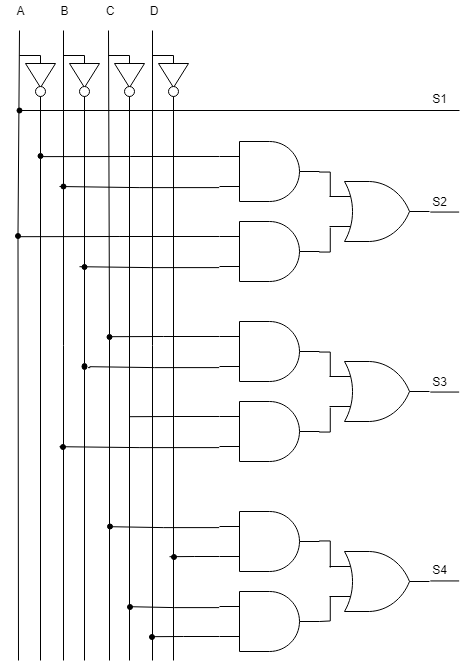
\includegraphics[width=0.8\textwidth]{./EJ_4/EJ4_TP1_Electro3.png}
    \caption{Circuito l\'ogico}
\end{figure}

\subsection{Programa en Verilog}
Se adjunta en la entrega de este trabajo pr\'actico el programa que representa al circuito mostrado en la secci\'on previa.

%\input{appendix.tex}
%


\end{document}
